\newpage
\section{Continuous Learning}
\label{sec:continuous_learning}

Beim obigen Beispiel (Perceptron) wurde der Error berechnet indem der Vorhersagewert vom erwarteten Wert subtrahiert wurde.

In diesem Kapitel werden Ansätze angeschaut, welche auch schauen \textbf{wie weit weg} die Vorhersage war.

\subsection{Adaline}
%\begin{flushleft}

Adaline steht für \textbf{Adaptive Linear Neuron} und ist ein \textbf{supervised classification Algorithmus}. Adaline funktioniert wie folgt:

\begin{itemize}
  \item Die Elemente des Input-Vektors (Featurevektors) werden jeweils mit einem Gewicht multipliziert und aufsummiert.
  \item Die Summe (z) wird einer \textbf{Aktivierungsfunktion} übergeben, welche den Wert $\hat{y}$ erzeugt.
  \item $\hat{y}$ wird dann verwendet, um den \textbf{Fehler} bzw. das \textbf{Update für die Gewichte} zu berechnen.
  \item $\hat{y}$ wird zudem einer \textbf{Schwellwertfunktion} übergeben, welche die Features einer Klasse zuordnet.
\end{itemize}




\newcommand{\myThresholdFunction}{
\draw[thick] %(-2.25em,0em) -- (1.25em,0em) 
			 (-0.5em,1.25em) -- (-0.5em,-1.25em)
(-0.5em,1.25em) -- (0.5em,1.25em)
(-0.5em,-1.25em) -- (-1.5em,-1.25em)
;}


\begin{figure}[H]
\centering
\label{fig:perceptron}
\begin{tikzpicture}[
     % define styles 
     clear/.style={ 
         draw=none,
         fill=none
     },
     net/.style={
         matrix of nodes,
         nodes={ draw, circle, inner sep=10pt },
         nodes in empty cells,
         column sep=1.5cm,
         row sep=-9pt
     },
     >=latex
]
% define matrix mat to hold nodes
% using net as default style for cells
\matrix[net] (mat)
{
% Define layer headings
|[clear]| \parbox{1.3cm}{\centering Input\\layer} & 
|[clear]| \parbox{1.3cm}{\centering Gewichtete\\Summe} &
|[clear]| \parbox{1.3cm}{\centering Aktivierungs\\funktion} &
|[clear]| \parbox{1.3cm}{\centering Schwellwert\\Funktion} \\
         
$+1$  		& |[clear]| & Error     & |[clear]| \\
|[clear]| 	& |[clear]| & |[clear]| & |[clear]| \\
$x_{1}$  	& |[clear]| & |[clear]| & |[clear]| \\
|[clear]| 	& $\Sigma$  & $\phi$ & \myThresholdFunction \\
\vdots  	& |[clear]| & |[clear]| & |[clear]| \\
|[clear]| 	& |[clear]| & |[clear]| & |[clear]| \\
$x_{n}$  	& |[clear]| & |[clear]| & |[clear]| \\
};
\draw[->] (mat-2-1) -- node[above=1mm] {$w_{0}$} (mat-5-2);
\draw[->] (mat-4-1) -- node[above=1mm] {$w_{1}$} (mat-5-2);
\draw[->] (mat-6-1) -- node[above=1mm] {$\vdots$} (mat-5-2);
\draw[->] (mat-8-1) -- node[above=1mm] {$w_{n}$} (mat-5-2);
\draw[->] (mat-5-2) -- node[above=1mm] {$z$} (mat-5-3);
\draw[->] (mat-5-3) -- node[above=1mm] {$\hat{y}$} (mat-5-4);
\draw[->] (mat-5-3) -- node[above=1mm] {$$} (mat-2-3);
\draw[->] (mat-2-3) -- node[above=1mm] {Update Gewichte} (-2.5cm, 1cm);

\draw[->] (mat-5-4) -- node[right=2em] {$\begin{cases}
       		1 &  \\
       		0 &
    	\end{cases}$} +(2cm,0);
\end{tikzpicture}
\caption{Adaline als Model}
\label{fig:adaline_model}
\end{figure}


% ============================================
\newpage
\subsubsection{Adaline vs Perceptron}

Ähnlich wie der Perceptron ist Adaline ein Einzellayer neuronales Netzwerk. Der Hauptunterschied liegt auf der Aktivierungsfunktion phi $\phi(z)$


\begin{itemize}
  \item Der \textbf{Perceptron} aktualisiert die Gewichte nur, wenn eine falsche Vorhersage getroffen wurde. Zudem wird die Error-Funktion erst nach der \textbf{Schwellwertfunktion} aufgerufen. Somit wird ihr stets immer nur eine 0 oder 1 übergeben.
  \item \textbf{Adaline} hingegen aktualisiert die Gewichte basierend auf einer \textbf{stetigen} Funktion (continuous). Der \textbf{Aktivierungsfunktion $\phi$}
 \end{itemize}



Wie in Abbildung \ref{fig:adaline_vs_perceptron} ersichtlich ist, werden die Gewichte bei Adaline \textbf{vor} der Entscheidungsfunktion aktualisiert.

\begin{figure}[h!]
	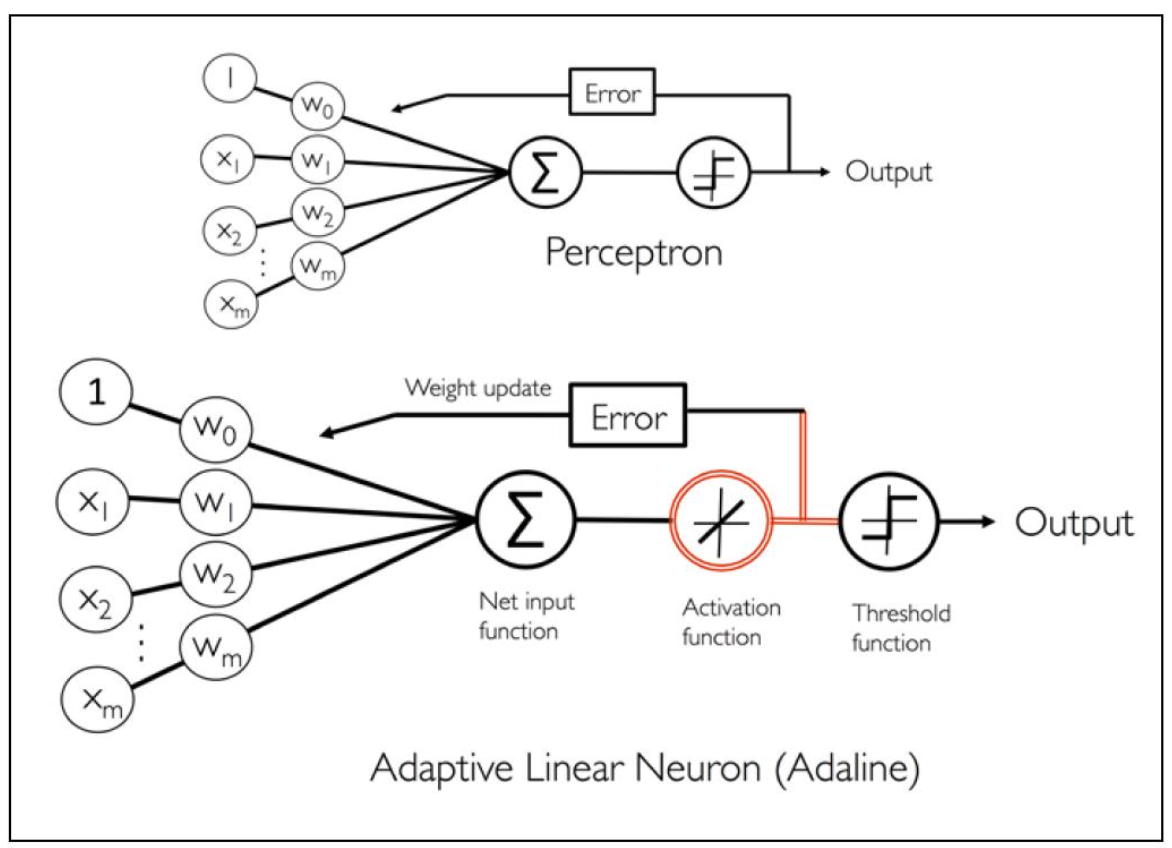
\includegraphics[scale=0.6]{figures/adaline_vs_perceptron}
	\caption{Adaline vs Perceptron}
	\label{fig:adaline_vs_perceptron}
\end{figure}

Im Gegensatz zum \textbf{binären Lernansatz} des Perceptron basieren viele supervised learning Algorithmen auf einer sogenannten \textbf{objective learning function}.


\newpage
\subsubsection{Objective Function}

Die Objective Function (Zielfunktion) ist mathematisch eine \textbf{Optimierung}.

Das Ziel hierbei ist es \textbf{optimale Parameter} zu finden. Optimal bedeutet den Output der Funktion entweder zu \textbf{maximieren} oder zu \textbf{minimieren}. 


Bei Machine Learning entsprechen die Parameter den \textbf{Gewichten}.


Eine Objective Funktion berechnet einen Output basierend auf den Eingaben:

\begin{itemize}
  \item Vorhersage (prediction)
  \item Eigentlicher Wert (labelled value)
\end{itemize}

Hierbei soll deren Differenz möglichst klein werden. Somit ist die Vorhersage sehr nahe am eigentlichen Wert. Ein Beispiel dafür zeigt Abbildung \ref{fig:objective_minimum}. 


\begin{figure}[h!]
	
\includegraphics[scale=0.4]{figures/objective_minimum}
	\caption{Beispiel Zielfunktion}
	\label{fig:objective_minimum}
\end{figure}



Objective Funktion ist ein sehr genereller Term im Bereich ML.
Meistens wollen wir den Output der Objective Funktion \textbf{minimieren}. In diesem Fall sprechen wir von einer \textbf{Cost Function} oder \textbf{Loss Function}.


Wollen wir den Output \textbf{maximieren} so sprechen wir von einer \textbf{Likelihood Maximization} Funktion.



 
\newpage
\subsubsection{Objective Function in Adaline}

Adaline verwendet die Cost Function \textbf{Sum of Squared Errors (SSE)}.

SSE summiert alle quadrierten Differenzen zwischen Vorhersage und effektivem Wert auf.

$$ SSE = \frac{1}{2} \sum_{i=1}^{m}(y^{(i)} - \hat{y}^{(i)})^{2} $$

Hier eine detailliertere Darstellung von $\hat{y}$

$$ SSE = \frac{1}{2} \sum_{i=1}^{m}(y^{(i)} - \phi(z^{(i)}))^{2} $$


Wichtig zu wissen:
\begin{itemize}
  \item Die Funktion SSE ist \textbf{differenzierbar (ableitbar)}. Daher kann für jeden Punkt die Steigung berechnet werden.
  \item Sie hat ein \textbf{globales Minimum}.
\end{itemize}


Diese beiden Punkte sind notwendig für \textbf{Optimierungsalgorithmen}. Diese helfen dabei den Wert der Gewichte zu bestimmen damit die Cost Function möglichst klein wird. (Bsp. Gradient Descent)


\subsubsection{Adaline Learning Rule}

$$ \Delta w_{j} = \eta \sum_{i=1}^{m} (y^{(i)} - \phi(z^{(i)})) * x_{j}^{(i)} $$


\begin{align*}
	\Delta w_{j}  &= \text{Gewichtsupdate} \\
	\eta &= \text{Learning Rate} \\
	m &= \text{Anzahl Samples}	\\
	y^{(i)} &= \text{Effektiver Zielwert (Label)} \\
	\phi &= \\
	z^{(i)} &= \\
	x_{j}^{(i)} &= \text{Feature j des Samples i} \\
\end{align*}


$$ w := w + \Delta w$$











TODO:
This update rule is in fact the stochastic gradient descent update for linear regression.[7]




